\documentclass[spanish,11pt,letterpaper]{article}

\usepackage[spanish]{babel}
\usepackage[utf8]{inputenc}
\usepackage{authblk}
\usepackage{amsmath}
\usepackage{amssymb}
\usepackage{amsthm}
\usepackage[margin=1in]{geometry}
\usepackage[title]{appendix}
\usepackage{graphicx}
\usepackage{hyperref}
% \usepackage{listings}
% \usepackage{xcolor}

\renewcommand{\vec}[1]{\mathbf{#1}}
\DeclareMathOperator*{\argmax}{arg\,max}
\decimalpoint

\title{Sistema de clasificación automática de documentos\\
Clasificación de canciones por género en base a la letra}
\author{Hernández Chiapa David Felipe\\
López García Gilberto Isaac}
\affil{Facultad de Ciencias\\{\small Universidad Nacional Autónoma de México}}
\date{\small\today}

\begin{document}

\maketitle

\section{Introducción}

Los géneros musicales varian mucho de unos a otros, por los ritmos, los instrumentos musicales
usados, la manera en que se canta y también en lo que se canta. Las letras de las canciones, pueden
variar mucho de género a género, incluso se podréa llegar a pensar que en los géneros más
relajados, sean estos Pop, Country, etc., se usen palabras agradables como ‘love’, mientras que del
otro lado en géneros como el Heavy Metal, se usen palabras más agresivas, como ‘hate’ o ‘death’.
He aquí la motivación para generar un clasificador de letras de canciones para determinar el género de
estas. Para lograr esto se usarán algoritmos especiales para clasificación, como lo son Bayes
Ingenuo y los árboles de decisión J48. De igual manera se describirán los problemas que se
fueron suscitando a lo largo de la implementación de este proyecto, y una explicación de por qué
la clasificación de letras de canciones representa un problema complicado.

\section{Descripción del problema}

La clasificación de textos o documentos consiste en que dado un conjunto de textos disponibles,
sean estos artículos científicos, artículos de revistas y en nuestro caso, canciones, se puedan
agrupar en cierta cantidad de grupos, temas o géneros. En nuestro caso, el problema que se busca
solucionar es el siguiente: Dado un conjunto de letras de canciones, ¿a que género pertenece cada
una?

Existen varios factores que hacen que este problema sea difícil de resolver, como lo son las
palabras usadas en cada género, la cantidad de contracciones y modismos regionales usados en ciertos géneros,
inclusive la cantidad de palabras. Un ejemplo parecido a lo que intentamos hacer, sería tomar
poemas de distintas épocas de la humanidad y tratar de clasificarlos por movimientos culturales, es
decir, si es del Renacimiento, del Barroco, etc., ya que cada movimiento tenía su propia métrica,
temas, y forma de escribir. Este tipo de problemas llegan a ser complicados, incluso para los
humanos, y probablemente lo es más para canciones, ya que el género de estas depende del ambiente
que generen y es posible que esto no solo dependa de la letra, sino, también de la música.

Se debe mencionar que lo que estamos tratando de lograr es aprendizaje, es decir, dado el conjunto
de letras de canciones, se buscarán patrones para que cuando se ingrese una letra nueva, el sistema
pueda clasificar de manera adecuada. Estos patrones los obtenemos por medio del aprendizaje
supervisado, al generar nuestro árbol de decisión, clasificador probabilístico,
o cualquier otro algoritmo de aprendizaje
supervisado. Se denomina supervisado porque los algoritmos se ejecutan usando un conjunto de
entrenamiento ya clasificado, que son datos que nosotros podemos definir, y que el algoritmo debe
aprender a, o entender cómo clasificar, para que nuestro algoritmo sepa qué hacer con datos
que no ha visto.

Requerimos de un agente inteligente ya que no solo nos interesa que clasifique la primera
ronda de letras de canciones, es decir, el conjunto de entrenamiento, sino que pueda seguir
clasificando letras que no ha visto como ya se dijo, e inclusive vuelva la clasificación
más eficiente. En otras palabras, nos interesa que aprenda a diferenciar canciones determinando
aquellas propiedades importantes que le ayudarán a lograr tal tarea.

En este artículo buscamos dar solución a este problema usando el aprendizaje supervisado, entrenando
el algoritmo con letras de canciones ya clasificadas por género musical. Existen
diversos algoritmos que cumplen esta propiedad de ser supervisados, como lo son Naive
Bayes, máquinas de soporte vectorial, etc. Aquí hacemos referencia a dos de estos,
árboles de decisión J48 y Naive Bayes.

\section{Descripción de la técnica elegida}

\subsection{Bayes Ingenuo}

Bayes Ingenuo, o Naive Bayes en inglés, es una técnica de aprendizaje supervisado para construir un
clasificador probabilístico. Este método ve las características del los objetos a clasificar y considera que la
probabilidad de estas caracteristicas es independiente de las demás características, es decir, el
hecho de que cierta palabra aparezca en un texto le da cierta probabilidad de pertenecer a cierto
género o géneros independientemente si las demás características para ser de ese género estan o no
presentes.

\subsubsection{Teorema de Bayes e independencia condicional}

El Teorema de Bayes dice que si $A,B$ son eventos, $\mathbb{P}[B] \neq 0$,
entonces \[ \mathbb{P}[A|B] = \frac{\mathbb{P}[B|A]\mathbb{P}[A]}{\mathbb{P}[B]}. \]

Dos eventos $A,B$ son independientes si $\mathbb{P}[A,B] = \mathbb{P}[A]\mathbb{P}[B]$.
De igual manera, $A$ y $B$ son condicionalmente independientes dado un evento $C$
si $\mathbb{P}[A,B|C] = \mathbb{P}[A|C]\mathbb{P}[B|C]$, esto se sigue de que la
probabilidad condicional es una probabilidad.

\subsubsection{Algoritmo}

Dado un vector $\vec{x} = (a_1,\ldots,a_n)$ de $n$ características, se le asigna
una probabilidad de pertenecer a una clase $C_i$ de entre $k$ clases
$\mathbb{P}[C_i|a_1,\ldots,a_n] = \mathbb{P}[C_i|\vec{x}]$\footnote{Abuso de notación.},
esto es igual a $\mathbb{P}[C_i,\vec{x}]/\mathbb{P}[\vec{x}]$.
El modelo asumen que los atributos de $\vec{x}$ son condicionalmente independientes
cuando se observa la categoría $C_i$ (de aquí el nombre ingenuo), entonces,
por Teorema de Bayes tenemos que
\begin{equation}
\mathbb{P}[C_i|\vec{x}] = \frac{\mathbb{P}[\vec{x}|C_i]\mathbb{P}[C_i]}{\mathbb{P}[\vec{x}]}
= \frac{\prod_j \mathbb{P}[a_j|C_i]\mathbb{P}[C_i]}{\mathbb{P}[\vec{x}]}.
%= \frac{\mathbb{P}[C_i]\prod_j \mathbb{P}[a_j|C_i]}{\sum_r \mathbb{P}[\vec{x}|C_r]\mathbb{P}[C_r]}
\end{equation}

Con estas probabilidades, dado un vector de entrada $\vec{x}$, el clasificador
decide la categoría $C_i$ a la que pertenece con la siguiente regla
\[ C_i = \argmax_{C_k} \mathbb{P}[C_k|\vec{x}] = \argmax_{C_k} \mathbb{P}[C_k]\prod_j \mathbb{P}[a_j|C_k], \]
nótese que no es necesario considerar $\mathbb{P}[\vec{x}]$ pues sólo depende
de $\vec{x}$, por lo que se puede considerar una constante de reescalamiento.

\subsubsection{Espacio de Hipótesis}

El espacio de hipótesis consiste de las funciones de probabilidad que satisfacen
la ecuación (1), el cual es infinito no numerable por ser la probabilidad una
medida sobre $[0,1]$, aún cuando el dominio de los datos se finito (y por ende
cualquier $\sigma$-álgebra sobre el dominio).

\subsubsection{Ventajas y desventajas}

Las ventajas del algoritmo son que es bastante sencillo, sólo son cuentas sobre
probabilidades que se tienen de antemano. Si la hipótesis de independencia
condicional realmente es válida, el algoritmo clasificará correctamente los
ejemplares rápidamente sin necesidad de tanto entrenamiento, y aún cuando
no se cumpla dicha hipótesis en la práctica ha demostrado tener muy buen
desempeño.

Una desventaja es que la hipótesis de independencia es muy fuerte y el clasificador
obviará relaciones entre las características de los ejemplares de entrada. También
requiere saber mucha información, las probabilidades \textit{a priori} de los datos
(pertenecer a una clase $C_k$, observar un ejemplar $\vec{x}$ de manera
independiente y dada una clase $C_k$), que si se calculan con una aproximación
frecuentista en datos no representativos hará que las probabilidades tiendan a 0
o 1 resultando en un pobre desempeño. Por esto mismo también le es difícil trabjar
a la computadora con atributos continuos.

\subsection{Árboles de decisión para clasificación}

Los árboles de decisión para clasificación son una herramienta de aprendizaje
supervisado para clasificación de ejemplares en categorías en base a los
atributos de los ejemplares, esto es, decide a qué categoría pertenece el
ejemplar. El árbol es una función que recibe un vector de atributos (o características) que
representan una instancia de un fenómeno o situación, realiza una serie de
preguntas sobre los valores de dichos atributos y con esta información
decide a qué categoría pertenece.

\subsubsection{Espacio de hipótesis}

Un árbol de decisión es una
función que dado un vector de $n$ características $\vec{x} = (a_1,\ldots,a_n)$,
donde cada característica toma valores en un conjunto finito $A_i$, decide si
pertenece a una de $k$ categorías distintas, esto es, asigna a $\vec{x}$ un
valor en $\{0,\ldots,k-1\}$. Así, los árboles de decisión son funciones de tipo
$A_1\times\ldots\times A_n \rightarrow \{0,\ldots,k-1\}$, la cardinalidad de este
conjunto es \[ k^r, r = \prod_{t=1}^n|A_t|, \] sin embargo, puede haber distintos
árboles que calculen la misma función, por ejemplo, cambiando el orden de las
preguntas sobre los atributos de $\vec{x}$. Así, el
espacio de hipótesis es el conjunto de árboles de decisión que calculan dichas
funciones sobre vectores de $n$ características, que tiene cardinalidad
al menos $k^r$.

\subsubsection{Entropía de una variable aleatoria e Información mútua}

La \textit{entropía} de una variable aleatoria $X$ es una medida de la cantidad
promedio de información que nos da $X$ cada vez que toma un valor, esto es, ocurre el evento
$X = x_s$. Un evento que ocurre con probabilidad 1 no nos da
información porque sabemos que va a ocurrir, pero si un evento con baja probabilidad
ocurre nos da más información sobre el fenómeno que modela $X$ en ese momento, entonces
la cantidad de información está relacionada con el inverso de la probabilidad
de ocurrencia.

Considera una variable aleatoria discreta $X$ que toma valores en un conjunto
finito $\{x_1,\ldots,x_k\}$ con probabilidad $p_s = \mathbb{P}[X = x_s]$. Definimos la
cantidad de información ganada al observar el evento $X = x_s$
como \[ I(x_s) := \log \left(\frac{1}{p_s}\right) = -\log(p_s).\footnote{La
base del logaritmo es arbitaria, cuando es 2 la unidad de medición son bits.} \]

La anterior definición cumple lo siguiente:
\begin{enumerate}
  \item Si $p_s=1$, $I(x_s) = 0$. Un evento que siempre ocurre no da información,
  \item $I(x_s) \geq 0$. La ocurrencia del evento $X = x_s$ da algo o nada de información,
  no hay pérdida,
  \item Si $p_i < p_j$, $I(x_i) > I(x_j)$. Eventos menos probables dan más información.
\end{enumerate}

Entonces, la entropía de $X$ se define como
\[ H_X := \mathbb{E}[I(x_s)] = \sum_{s=1}^k p_sI(x_s) = -\sum_{s=1}^k p_s\log(p_s).
\footnote{Consideramos $0\log(0)=0$.} \]

La extropía está acotada por $0 \leq H_X \leq \log(k)$. Es 0 cuando un evento
ocurre con probabilidad 1 y los demás con probabilidad 0 pues no ganamos información,
siempre ocurre lo mismo. Es $\log(k)$ cuando todos los eventos son equiprobables
y la incertidumbre es máxima.

Dadas dos variables aleatorias discretas $X,Y$, la \textit{información mútua} es
una medida de la información que $X$ y $Y$ comparten, esto es, cuánto se reduce
la incertidumbre de una cuando se observa la otra. Se define como
%\[I(X;Y) := \sum_{t=1}^l\sum_{s=1}^k p_{X,Y}(s,t)\log\left(\frac{p_{X,Y}(s,t)}{p_X(s)p_Y(t)}\right),\]
%donde $p_{X,Y}$ es la función de masa conjunta. Esto también puede escribirse como
\[I(X;Y) := H_Y-H_{Y|X} = H_X-H_{X|Y},\]
donde $H_{Y|X}$ es la entropía de $Y$ después de observar $X$.

\subsubsection{Algoritmos ID3 y J48}

El algoritmo ID3 de Ross Quinlan genera árboles de decisión buscando minimizar la
cantidad de preguntas sobre los atributos de un vector de entrada que deben hacerse
para decidir su clasificación seleccionando los atributos más importantes,
los que dan más información sobre el problema. Para determinar qué características son
las más importantes, busca maximizar información obtenida al observar una
característica.

Cuando un árbol pregunta sobre un atributo $E$, el conjunto de ejemplares $X$ con
etiquetas $Y$ es dividido en subconjuntos $X_1,\ldots,X_k$ (con sus correspondientes
eqiquetas $Y_1,\ldots,Y_k$) donde el atributo $E$ de todos los ejemplares en $X_i$
es $i$, para cada valor $i$ de $E$. Maximizar la
\textit{ganancia de información} es encontrar el atributo $E$ tal que la diferencia
en la entropía de $X$ antes y después de dividir el conjunto de ejemplares es
máxima:
\[\argmax_E IG(E),\]
donde
\[IG(E) := H_X - H_{X|E} = H_X - \sum_{i=1}^k \frac{|X_i|}{|X|}H_{X_i}\]
es la ganancia de información al preguntar por el atributo $E$. Aquí entiéndase
$H_X$ en términos de $I(y_i)$ la información que da un ejemplar de $X$ que tiene
etiqueta $y_i \in Y$ (pertenece a la categoría $i$). Como
información mútua, $IG(E)$ nos dice cuánto se reduce la incertidumbre en $X$ después
de observar a $E$.

El algoritmo ID3 construye el árbol de decisión como sigue:
\begin{enumerate}
  \item Si todos los ejemplares de $X$ pertenecen a la misma categoría $i$ crea un nodo con etiqueta $i$.
  \item Si ya no quedan atributos para preguntar crea un nodo con la etiqueta de la categoría más común en $X$.
  \item Encuentra el atributo $E$ que maximiza $IG(E)$ y crea un nuevo árbol de decisión con raíz $E$. Para cada valor $e$ que pueda tomar $E$ y generar los subconjuntos $X_e$ y para cada $e$:
  \begin{enumerate}
    \item Si $X_e = \varnothing$ añadir una rama $E=e$ al árbol con raíz $E$ y un nodo con etiqueta la categoría más común en $X$.
    \item Añadir una rama $E=e$ al árbol con raíz $E$ y subárbol el árbol resultante de ID3 sobre el conjunto $X_e$ (sin tomar en cuenta el atributo $E$).
  \end{enumerate}
  \item Regresar el árbol con raíz $E$.
\end{enumerate}

El algoritmo J48 de Weka es una mejora sobre el algoritmo ID3\footnote{La versión libre del
algoritmo C4.5 de Ross Quinlan.}. Permite trabajar con atributos continuos determinando
un umbral para la separación del conjunto de ejemplares (ejemplo,
atributo numérico $r$ y umbral $t$, genera subconjuntos $X_{r\leq t},X_{r > t}$). También puede
trabajar con datos incompletos (los ignora). J48 genera un árbol de decisión de
la misma manera que ID3 pero después de crearlo procede a podarlo eliminando ramas
que no contribuyen al resultado de la clasificación de ejemplares.

\subsubsection{Ventajas y desventajas}

Los árboles de decisión son herramientas sencillas, solo realizan una serie de
preguntas sobre los atributos de los ejemplares (¿qué valor tiene?) por lo que
su funcionamiento es fácil de comprender y no son muy exigentes computacionalmente,
escpecialmente cuando toman en cuenta pocos atributos para una clasificación
(lo suficientemente) exitosa.

Por otro lado, los árboles de decisión sufren de sobreentrenamiento cuando no
fue posible encontrar patrones en los datos de entrenamiento al generarlo, obteniendo árboles
grandes y complicados que no generalizan. También, una vez construido el modelo
es difícil modificarlo, por lo que habrá que construir un nuevo árbol para nuevos
datos (esto es, no permite \textit{online learning}).

\section{Descripción de la propuesta e implementación}

Para resolver este problema proponemos el uso de dos clasificadores para realizar
una comparación en desempeño, árboles J48 y Bayes Ingenuo como ya se mencionó. Dos
algoritmos que no requieren de mucha parametrización y son fáciles de construir
usando la biblioteca de Machine Learning, Weka. Los modelos serán entrenados
y evaluados utilizando la técnica de validación cruzada en 10 iteraciones para
evitar que los resultados sean dependientes de la partición de los datos de entrada.

\subsection{Datos}

Los datos para trabajar son la letra de canciones y el género asignado a la canción,
obtenidos de la base de datos del servicio de letras musicales y traducción
Musixmatch.\footnote{\url{http://www.musixmatch.com/}.}

Usando un plan de servicio gratuito para testing sólo tenemos acceso al 30\% de
la letra de cada canción. Mediante un wrapper de Python,
pymusixmatch\footnote{\url{https://github.com/hudsonbrendon/python-musixmatch}},
realizamos llamadas a la API de Musixmatch para obtener las canciones más populares
de ciertos países (BE, CA, DE, GB, MX, NO, RU, SE, US, AU, AE, CH, UG, NZ).

Se filtraron canciones para quedarnos sólo con aquellas que tenían un género musical
asignado y letra de la canción en inglés, eliminando elementos repetidos.
Más aún, había géneros musicales con pocas canciones, por lo que se eliminaron
canciones cuyo género tuviera menos de 10 canciones en el conjunto. El conjunto final
de datos consta de 575 canciones (la letra y el género de) de una cantidad
inicial de 1504.

Durante la solicitud de los datos, se eliminaron las dos últimas líneas de la letra, que
es un mensaje de Musixmatch comunicando que el dato no es para uso comercial.
La etiqueta de cada canción es \texttt{CN} donde \texttt{N} es el id del género
asignado por Musixmatch. Durante la solicitud de los datos se generó un diccionario
que contiene el id y el nombre del género en texto de los datos finales,
puede encontrarse en el Apéndice A.

\subsubsection{Preprocesamiento}

Durante la solicitud de los datos se decidió eliminar comillas dobles (\texttt{"}),
pues su uso era escaso y delimitaban frases pequeñas.

Para procesar las letras
es necesario representar el texto (en minúsculas) como vectores de entradas numéricas usando
el modelo de Weka, \texttt{StringToWordVector}. El modelo fue creado usando como
delimitadores para el tokenizer
``\texttt{\textvisiblespace\textbackslash r\textbackslash t.,;:\char`\"}%
\texttt{'‘’`()¿?!$\cdot*+-/\{\}$[]$<>$@\textbackslash n}'', generando palabras (unigramas).
Los datos incluyen gran cantidad de contracciones, \textit{slangs} y sonidos escritos, por
lo que obviamos signos de puntuación, tipos de paréntesis y símbolos poco comunes
que llegan a aparecer. Aunque las comillas simples se usan en contracciones y
modifican el significado de las palabras decidimos eliminarlas porque los datos
no son consistentes, ``you're'' llegó a aparecer como ``you\textvisiblespace re''
o con otro tipo de comillas simples que se identifican como caracteres distintos.
También se solían usar las comillas simples en modismos ('bout
en vez de about, runnin' para running) pero no en todas las canciones (gon,gon',gonna
aparecían). Todo esto generaba ruido en los datos y aumentaba el número de
características de la representación en vectores.

También se utilizó un stemmer, el modelo \texttt{IteratedLovinsStemmer} que analiza
prefijos para identificar raíces y palabras similares%
\footnote{A diferencia de \texttt{SnowballStemmer} que simplifica
la palabra eliminando sufijos hasta encontrar la raíz. Por modismos
y contracciones el algoritmo es inapropiado en este caso, aún cuando el idioma
de las letras es el inglés.}.

Finalmente, la lista de \textit{stopwords} utilizada fue \texttt{Rainbow}, además
se eliminaron manualmente tokens que consistían de números posiblemente seguidos de letras
(100k, 7am, etc.) y tokens de dos caracteres que normalmente sobran por quitar
comillas simples (``re'' de ``you're'' por ejemplo).

\subsection{Clasificación}

Como primera aproximación tratamos de clasificar las canciones mediante las
palabras que aparecen en su letra, una idea que surge de pensar que la
naturaleza del género reside en el ambiente que genera la canción entre la música
y letra, por ejemplo,
esperamos que el Pop cree un ambiente más amable y alegre comparado con Heavy
Metal sombrío, pensamos que encontraremos palabras como `love' y `happiness' en Pop,
`hate' y `death' en Heavy Metal, `rave' y `party' en EDM, etcétera. Podríamos esperar
entonces que un árbol de decisión sea capaz de encontrar tales patrones en los
textos y decida correctamente el género a partir de vectores booleanos (la
palabra figura en la cacnión o no).

Un problema con esto es que subgéneros toman elementos de otros
géneros por lo que pensar
que un conjunto de palabras aparecen exclusivamente en un género es una intuición errónea,
por lo que para refinar la idea anterior podemos contar las ocurrencias de las palabras
y que estas cantidades sean las características de los vectores de entrada.

Entonces, la propuesta consiste en usar dos representaciones para el texto,
vectores booleanos y vectores que cuentan ocurrencias de palabras, y usar dos
modelos de clasificadores para intentar identificar el género de la canción.

\section{Resultados}

\subsection{Pruebas preliminares}

Realizando experimentos para observar el comportamiento de los modelos
de Weka refinamos un poco el modelo. Empezamos utilizando el stemmer
\texttt{SnowballStemmer} ya que implementa el algoritmo de Porter para encontrar
raíces en texto en inglés, pero esto resultó en vectores con muchas características,
por lo que rápidamente fue descartada esta idea y escogimos
\texttt{IteratedLovinsStemmer} por considerarlo más adecuado a este problema.

\begin{center}
\begin{tabular}{c | c}
Stemmer &  \# de características (c/género)\\
\hline
Sin Stemmer (\texttt{NullStemmer}) & 3840\\
\texttt{SnowballStemmer} & 3840\\
\texttt{IteratedLovinsStemmer} & 2860
\end{tabular}
\end{center}

En la tabla anterior puede apreciarse la diferencia entre los stemmers. Como se
mencionó en la sección 4.1.1, el algoritmo de \texttt{IteratedLovinsStemmer}
se desempeña mejor por las irregularidades lingüísticas de los datos.

Añadiendo como lista de \textit{stopwords} \texttt{Rainbow}, hay una reducción de
198 atributos, esto es, 2662 características incluyendo el género. Eliminando números
y palabras de 2 caracteres con la expresión regular \texttt{[0-9]+[a-z]*|[a-z][a-z]}
reducimos el número de características a 2503. Una vez reducido en 1337 el número de
características de los vectores hacemos el trabajo de los clasificadores más
fácil pues no tendrán que considerar elementos sin significado (principalmente
para estructura gramatical del lenguaje) para clasificar y evitar sobreentrenamiento.

\subsection{Primer intento de clasificación}

Entrenando un árbol de decisión J48 y un clasificador Bayesiano ingenuo con los
parámetros por defecto especificados por Weka obtenemos los siguientes resultados

\begin{center}
\begin{tabular}{c | c | c}
Clasificador &  \# de aciertos (Total 575) & \% de aciertos \\
\hline
Bayes Ingenuo (booleano) & 187 & 32.5217\% \\
Bayes Ingenuo (ocurrencias) & 219 & 38.087\% \\
J48 (booleano) & 219 & 38.087\% \\
J48 (ocurrencias) & 199 & 34.6087\%
\end{tabular}
\end{center}

Un comportamiento observado en la matriz de confusión de los 4 clasificadores fue
que las canciones de Pop, que son los datos más abundantes con 266 instancias comparado
con 83 instancias del segundo género más popular Alternative (Rock alternativo),
estaba afectando mucho a los clasificadores pues muchas canciones de otros géneros
eran calsificadas como Pop y muchas canciones de Pop (al rededor de 100) se
clasificaban dentro de otros géneros, como se ve en las Figuras 1 y 2.

\begin{figure}[h]
\centering
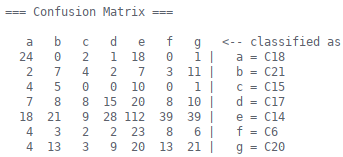
\includegraphics[width=0.35\textwidth]{bayes_boolean}
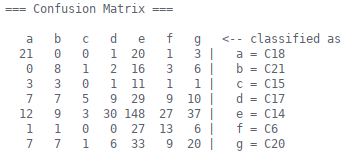
\includegraphics[width=0.35\textwidth]{bayes_counter}
\caption{Matrices de confusión. Bayes booleano (izq.) y Bayes ocurrencias (der.)}
\end{figure}
\begin{figure}[h]
\centering
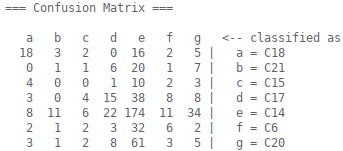
\includegraphics[width=0.35\textwidth]{j48_boolean}
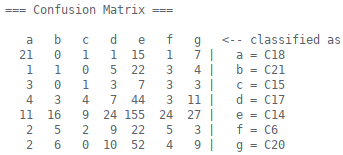
\includegraphics[width=0.35\textwidth]{j48_counter}
\caption{Matrices de confusión. J48 booleano (izq.) y J48 ocurrencias (der.)}
\end{figure}

\subsection{Segundo intento de clasificación}

Dado que las canciones de Pop eran las que más abundates y eran los ejemplares
donde más se equivocaban los clasificadores intentamos eliminar 166 canciones de
Pop para nivelar un poco la distribución de los datos y realizando el mismo
procedimiento esperando una mejora en la clasificación, pero de hecho, empeoró
la precisión de los algoritmos:

\begin{center}
\begin{tabular}{c | c | c}
Clasificador &  \# de aciertos (Total 398) & \% de aciertos \\
\hline
Bayes Ingenuo (booleano) & 97 & 24.3719\% \\
Bayes Ingenuo (ocurrencias) & 123 & 30.9045\% \\
J48 (booleano) & 96 & 24.1206\% \\
J48 (ocurrencias) & 89 & 22.3618\%
\end{tabular}
\end{center}

\begin{figure}[h]
\centering
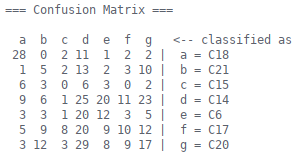
\includegraphics[width=0.35\textwidth]{bayes_spop_boolean}
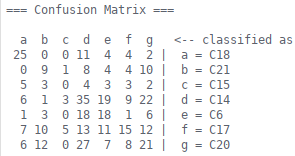
\includegraphics[width=0.35\textwidth]{bayes_spop_counter}
\caption{Matrices de confusión. Bayes booleano (izq.) y Bayes ocurrencias (der.)}
\end{figure}
\begin{figure}[h]
\centering
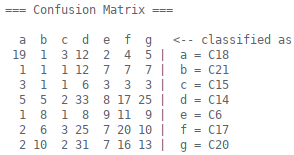
\includegraphics[width=0.35\textwidth]{j48_spop_boolean}
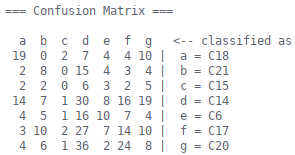
\includegraphics[width=0.35\textwidth]{j48_spop_counter}
\caption{Matrices de confusión. J48 booleano (izq.) y J48 ocurrencias (der.)}
\end{figure}

\section{Conclusiones}

\begin{appendices}
\section{Diccionario de géneros}
\begin{center}
\begin{tabular}{|c|c|c||c|c|c|}
\hline
id & Género & \# canciones & id & Género & \# canciones\\
\hline
14 & Pop & 266 & 15 & R\&B/Soul & 20 \\
17 & Dance & 76 & 21 & Rock & 36 \\
18 & Hip Hop/Rap & 46 & 6 & Country & 48 \\
20 & Alternative & 83 & & & \\
\hline
\end{tabular}
\end{center}
\end{appendices}

\begin{thebibliography}{9}
\bibitem{russellnorvig}
Russell, S. J., \& Norvig, P. (2010).
\textit{Artificial intelligence: a modern approach}.
Upper Saddle River: Prentice-Hall.

\bibitem{haykin}
Haykin, S. S. (2011).
\textit{Neural networks and learning machines}.
New Dehli: PHI Learning.

\bibitem{bell}
Bell, J. (2015).
\textit{Machine learning: hands-on for developers and technical professionals}.
Indianapolis: John Wiley \& Sons.
\end{thebibliography}

\end{document}
